\begin{tabular}{m{30mm}m{20mm}m{60mm}}
	\begin{tikzpicture}
		% draw the background cylinder
		\bgcylinder{0,0}{5.8}{1.5}{.4}{color1}{color1}

		% label some coordinates for use later
		\coordinate (f) at (1.5, 3.6) {};
		\path (f) -- ++(-0.3, 0.5) coordinate (ful);
		\path (f) -- ++(0.3, 0.5) coordinate (fur);
		\path (f) -- ++(-0.3, -0.5) coordinate (fdl);
		\path (f) -- ++(0.3, -0.5) coordinate (fdr);

		% draw theta	
		\begin{pgfonlayer}{foreground}
			\drawtheta{(f)}{-1.0}{1}{th}{}
		\end{pgfonlayer}

		% draw the strings and color the S region
		\filldraw[color2fill] (f) to[out=-135, in=90] (fdl) -- (fdl |- thL) -- node[ed,pos=1]{$M$} ++(0, -0.8) arc (0:-180:0.3) -- node[ed,pos=0]{$M^*$} ++(0, 0.2) to[out=90, in=-90] (thL) -- (thL') -- (thL' |- bot') -- (thR' |- bot') -- (thR') -- (thR) to[out=90, in=-90] ++(-0.6, 0.6) -- ($(fur) + (0.6, 0)$) -- node[ed,swap,pos=1]{$M^*$} ++(0, 0.2) arc(0:180:0.3) -- node[ed,swap,pos=0]{$M$} (fur) to[out=-90, in=45] (f);
		\draw[ds] (f) to[out=135, in=-90] (ful) -- node[ed]{$Q$} (ful |- ul);
		\draw[ds] (f) to[out=-45, in=90] (fdr) -- node[ed,near end]{$P$} (fdr |- bot);

		% draw nodes and label regions	
		\node[vert] at (f) {$f$};
		\node[anchor=north west,color1dark,re] at ($(ul)!.05!(dl)$) {$R$};
		\node[anchor=south east,color2dark,re] at (dr) {$S$};
	\end{tikzpicture}
	& \begin{center} = \end{center} &
	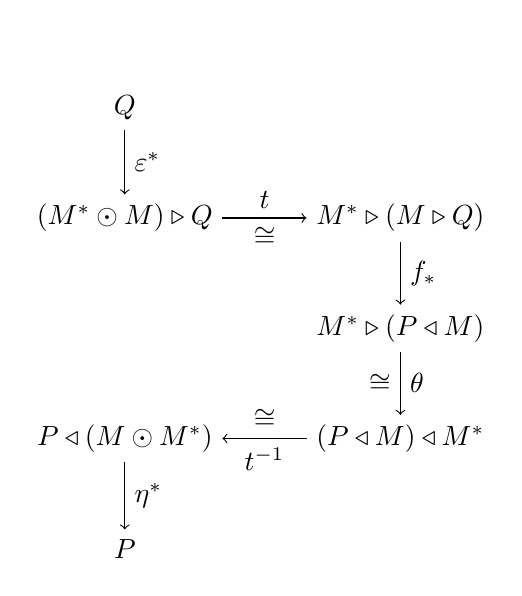
\begin{tikzpicture}
		\node at (0, 6.5) {}; % to help align the bottom of this picture with the bottom of the string diagram
		\node (A) at (0, 5.6) {$\lsh{Q}$};
		\node (B) at (0, 4.2) {$\lsh{(M^* \odot M) \triangleright Q}$};
		\node (C) at (3.5, 4.2) {$\lsh{M^* \triangleright (M \triangleright Q)}$};
		\node (D) at (3.5, 2.8) {$\lsh{M^* \triangleright (P \triangleleft M)}$};
		\node (E) at (3.5, 1.4) {$\lsh{(P \triangleleft M) \triangleleft M^*}$};
		\node (F) at (0, 1.4) {$\lsh{P \triangleleft (M \odot M^*)}$};
		\node (G) at (0, 0) {$\lsh{P}$};

		\draw[->] (A) -- node[right]{$\lsh{\varepsilon^*}$} (B);
		\draw[->] (B) -- node[above]{$\lsh{t}$} node[below]{$\cong$} (C);
		\draw[->] (C) -- node[right]{$\lsh{f_*}$} (D);
		\draw[->] (D) -- node[right]{$\theta$} node[left]{$\cong$} (E);
		\draw[->] (E) -- node[below]{$\lsh{t^{-1}}$} node[above]{$\cong$} (F);
		\draw[->] (F) -- node[right]{$\lsh{\eta^*}$} (G);
	\end{tikzpicture}
\end{tabular}
